\documentclass[tikz]{standalone}

\usepackage{tikz}
\usetikzlibrary{positioning, arrows.meta, shapes, snakes, shadings}
\usepackage{amsmath,amssymb,amsthm,pgfplots}

\begin{document}

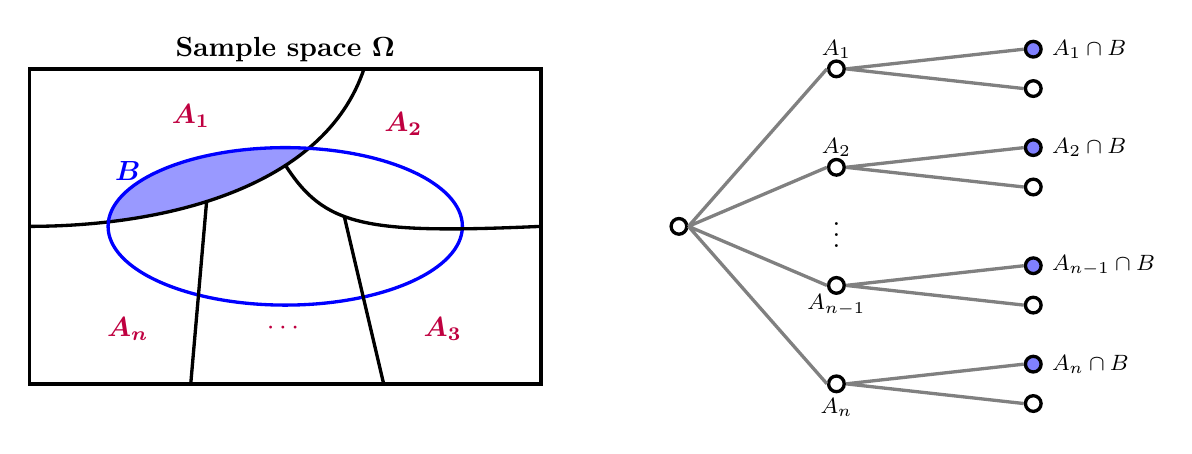
\begin{tikzpicture}
    %% left
    \begin{scope}
        \clip (0,0) circle [x radius=2.25, y radius=1];
        \fill[fill=blue!40] (-3.25,0) .. controls (-1.5,0) and (0.5,0.5) .. (1,2);
    \end{scope}
    \draw[very thick] (-3.25,-2) rectangle (3.25,2);
    \draw[very thick] (-3.25,0) .. controls (-1.5,0) and (0.5,0.5) .. (1,2);
    \draw[very thick, blue] (0,0) circle [x radius=2.25, y radius=1] (-2,0.7) node {\color{blue} $\boldsymbol{B}$};
    
    \draw[very thick] (0,0.78) .. controls (0.5,0) and (1,-0.1) .. (3.25,0)
                  (0.75,0.125) -- (1.25,-2)
                  (-1,0.3) -- (-1.2,-2);
    \draw (0,2.25) node {\textbf{Sample space $\boldsymbol{\Omega}$}};
    \draw (-1.2,1.4) node[purple] {$\boldsymbol{A_1}$}
      (1.5,1.3) node[purple] {$\boldsymbol{A_2}$}
      (2,-1.3) node[purple] {$\boldsymbol{A_3}$}
      (0,-1.3) node[purple] {$\cdots$}
      (-2, -1.3) node[purple] {$\boldsymbol{A_n}$};
      
    %% right tree
    \draw[very thick] (5,0) node[draw, circle, inner sep=2pt] (s1) {}
    
                      (7,2) node[draw, circle, inner sep=2pt] (s21) {}
                      (7,0.75) node[draw, circle, inner sep=2pt] (s22) {}
                      (7,-0.75) node[draw, circle, inner sep=2pt] (s23) {}
                      (7,0) node {$\boldsymbol{\vdots}$}
                      (7,-2) node[draw, circle, inner sep=2pt] (s24) {}
                      
                      (9.5,2.25) node[draw, circle, inner sep=2pt, fill=blue!50] (s31) {}
                      (9.5,1.75) node[draw, circle, inner sep=2pt] (s32) {}
                      (9.5,1) node[draw, circle, inner sep=2pt, fill=blue!50] (s33) {}
                      (9.5,0.5) node[draw, circle, inner sep=2pt] (s34) {}
                      (9.5,-0.5) node[draw, circle, inner sep=2pt, fill=blue!50] (s35) {}
                      (9.5,-1) node[draw, circle, inner sep=2pt] (s36) {}
                      (9.5,-1.75) node[draw, circle, inner sep=2pt, fill=blue!50] (s37) {}
                      (9.5,-2.25) node[draw, circle, inner sep=2pt] (s38) {}
                      
                      (7,2.25) node {\footnotesize $A_1$}
                      (7,1) node {\footnotesize $A_2$}
                      (7,-1) node {\footnotesize $A_{n-1}$}
                      (7,-2.3) node {\footnotesize $A_n$}
                      (9.6,2.25) node[anchor=west] {\footnotesize $A_1 \cap B$}
                      (9.6,1) node[anchor=west] {\footnotesize $A_2 \cap B$}
                      (9.6,-0.5) node[anchor=west] {\footnotesize $A_{n-1} \cap B$}
                      (9.6,-1.75) node[anchor=west] {\footnotesize $A_{n} \cap B$};
    \draw[very thick, gray] (s1.east) -- (s21.west)
                            (s1.east) -- (s22.west)
                            (s1.east) -- (s23.west)
                            (s1.east) -- (s24.west)
                            (s21.east) -- (s31.west) (s21.east) -- (s32.west)
                            (s22.east) -- (s33.west) (s22.east) -- (s34.west)
                            (s23.east) -- (s35.west) (s23.east) -- (s36.west)
                            (s24.east) -- (s37.west) (s24.east) -- (s38.west);
\end{tikzpicture}
    
\end{document}